\documentclass[12pt,letterpaper,oneside]{book}
\usepackage{algpseudocode}
\usepackage{algorithm}
\usepackage{subfig}
\usepackage[hidelinks]{hyperref}
\usepackage{ThesisStyle/afitThesis}
\usepackage{Packages/sf298}
\usepackage[toc,page]{appendix}
\usepackage[normalem]{ulem}
\useunder{\uline}{\ul}{}
\usepackage{setspace}
\usepackage{listings}
\usepackage{color}
\definecolor{mygreen}{rgb}{0, 0.6, 0}
\definecolor{mygray}{rgb}{0.5, 0.5, 0.5} \definecolor{mymauve}{rgb}{0.58, 0, 0.82}

\lstset{ 
  backgroundcolor=\color{white},   % choose the background color; you must add \usepackage{color} or \usepackage{xcolor}; should come as last argument
  basicstyle=\footnotesize,        % the size of the fonts that are used for the code
  breakatwhitespace=false,         % sets if automatic breaks should only happen at whitespace
  breaklines=true,                 % sets automatic line breaking
  commentstyle=\color{mygreen},    % comment style
  extendedchars=true,              % lets you use non-ASCII characters; for 8-bits encodings only, does not work with UTF-8
  frame=single,	                   % adds a frame around the code
  keepspaces=true,                 % keeps spaces in text, useful for keeping indentation of code (possibly needs columns=flexible)
  keywordstyle=\color{blue},       % keyword style
  numbers=left,                    % where to put the line-numbers; possible values are (none, left, right)
  numbersep=5pt,                   % how far the line-numbers are from the code
  numberstyle=\tiny\color{mygray}, % the style that is used for the line-numbers
  rulecolor=\color{black},         % if not set, the frame-color may be changed on line-breaks within not-black text (e.g. comments (green here))
  showspaces=false,                % show spaces everywhere adding particular underscores; it overrides 'showstringspaces'
  showstringspaces=false,          % underline spaces within strings only
  showtabs=false,                  % show tabs within strings adding particular underscores
  stepnumber=2,                    % the step between two line-numbers. If it's 1, each line will be numbered
  stringstyle=\color{mymauve},     % string literal style
  tabsize=2,	                   % sets default tabsize to 2 spaces
  %title=\lstname                   % show the filename of files included with \lstinputlisting; also try caption instead of title
}


%% Customize your document with your personal information
%% First, comment out the appropriate document type
\afitthesis %%default
% \afitreport
% \dissertation
% \prospectus

\author{Lauren M. Bramblett}
\rank{2nd Lt, USAF}  % If a civilian, comment out this line. 

\docdesignator{AFIT-ENS-MS-19-M-XXX}
\department{Department of Operational Sciences}
\graduationdate{March 21, 2019}

\flytitle{Turbojet Range, Loiter, and Altitude Tradeoff Estimation in Efficient Modeling and Optimization Formulations} 
\title{\MakeUppercase{AFIT/ENS Thesis Primer:}\\
       \MakeUppercase{ a document in \LaTeX}}
                             % Note, if you use \MakeUppercase to put
                             % the title in all uppercase as the style
                             % guide demands, understand that the
                             % command does not allow page breaks ``\\'' 
                             % within its brackets.
\previousdegrees{B.S.}
\acdegree{Master of Science in Operations Research}
 
\committee{{Dr. L. E. Champagne\\Chair},
           {Dr. R. R. Hill\\Reader}
}

\address{2950 Hobson Way\\ Air Force Institute of Technology \\
Wright-Patterson AFB, OH 45433}

\distribution{DISTRIBUTION STATEMENT A\\[-10pt]
\MakeUppercase{Approved for Public Release; distribution unlimited.}
} 

\disclaimer{The views expressed in this document are those of the
author and do not reflect the official policy or position of the
United States Air Force, the United States Department of Defense or
the United States Government.  This material is declared a work of the
U.S. Government and is not subject to copyright protection in the
United States.}

% International students may consider using the following disclaimer
% statement: \dislaimer{The views expressed in this document are those
% of the author(s) and do not reflect the official policy or position
% of the United States Air Force, Department of Defense, United States
% Government, the corresponding agencies of any other government,
% NATO, or any other defense organization.}


\input{Thesis/Preamble/myFigures}
\title{TURBOJET RANGE, LOITER, AND ALTITUDE TRADEOFF ESTIMATIONS IN EFFICIENT MODELING AND OPTIMIZATION FORMULATIONS}


\begin{document}
\frontmatter
	\flyleaf
    \disclaimerpage
    \titlepageAFIT
    \committeepage
    \begin{abstract}
\hspace{0.5cm}Identifying accurate tradeoffs between loiter time, range, and loiter altitude for jet aircraft are critical for mission planning, but current methods are cumbersome and time and labor intensive. This research introduces a new method for determining tradeoffs between loiter time, range, and loiter altitude for jet aircraft utilizing specific aircraft performance characteristics and the Bréguet range and endurance equations. Results from this new methodology are compared to the existing model used by the National Air and Space Intelligence Center for flight planning. This method is then extended and applied to several routing assignment problems, taking advantage of the incorporation of performance characteristics in their formulation. Example problems are generated using binary integer programming models and nonlinear mixed integer programming models. 
\end{abstract}
    

%     As an AFIT graduate student, you are about to write one of the
%     longest documents of your career.  Whether you use a ``what you see
%     is what you get'' (WYSIWYG) interface like Microsoft Word
%     \trademark or a typesetting system like \LaTeX\ldots when you
%     create a digital document, you are writing a program.  The larger
%     any program is, the more bugs it will contain and the more likely
%     the program will result in a catastrophic error.  Common bugs
%     result in improper formating, double words, lost sentences,
%     and---in the worst case---corrupted, unreadable files.
% 
%     Typesetting systems such as \LaTeX\ limit the new lines of code
%     generated with each new document.  As a result, they produce
%     cleaner, easier-to-debug products.  Additional benefits of \LaTeX\
%     are rapid reformatting and high quality typesetting of equations
%     and vector graphics.

    \begin{acknowledgements}

\begin{center}
      \emph{Raisin Canes.}
\end{center}
 
Much thanks to everyone.  

\end{acknowledgements}




    \tableofcontents
    \listoffigures
    \listoftables
\mainmatter
	\chapter{Introduction}
	\section{Overview}
\hspace{.5cm} Range and loiter time have been explored in the field of aeronautics by many individuals and companies, seeking to maximize both separately. However, since there is little utility for such use in a commercial environment, the trade-offs of range and loiter time for an aircraft have not been widely explored. The National Air and Space Intelligence Center (NASIC) seeks an optimization tool that efficiently identifies the range, loiter time, and loiter altitude tradeoffs while minimizing error. Customers of NASIC are constructing aircraft mission plans and are looking for a spectrum of flight plans that meet their mission criteria. Analysts are currently using labor-intensive methods to provide range, radius, and time estimates for specific aircraft configurations. As a result, improved methods integrated into the process could result in significant time and cost savings. 

\section{Background}

\hspace{.5cm}The mission planning tool used by the National Air and Space Intelligence Center allows for a selection of aircraft, standardized load out, and flight profile. The outputs of the current tool are mission range or loiter time depending on initial user inputs and, depending on the feasibility of those inputs, may output an error. The program mainly operates from a fuel constrained perspective and provides the outputs based on fuel reserve after user-defined parameters such as warm up, take-off, cruise altitude, length of combat, and fuel reserve. \par
The high fidelity of the mission planning tool allows finding specific points, and a trade-off of loiter time and range by interpolating between these points, which are in close proximity. This aspect of finding the frontier of loiter time and range is time consuming and must be done by hand by analysts familiar with the mission planning tool. The intent to find a trade-off is similar to Snyder \cite{Tradeoffs} finding the performance tradeoffs in various rotocraft. Some have used the simplification of equations to maximize range \cite{breguetRangeEqn, OptimizeBreguet}, while Raymer \cite{LoiterTimeFromRange} found methods of approximating endurance from range at specific points. Extensions of this problem in Alighanbari et al \cite{Alighanbari} formulated an optimization problems with endurance constructed as an objective and timing as the constraints of multiple UAV control. 

\section{Motivation}
\hspace{.5cm}The current method of deriving an optimal range and loiter time for a customer with at least one given as a parameter gives results that are accurate within five percent of actual, but are time consuming and inefficient to calculate. Additionally, the sensitivity of the current problem is unknown, given that the current method requires tabular calculations. The use of goal programming and optimization methods are used to leverage the parameters in this dynamic problem and simplify the initial model. The geometric equivalence of the current solution method is used as a backbone for finding the vertical distance of two intersecting polynomials, representing aircraft's ingress to a range and egress to a base, using the result as an objective.\par
The primary objective of this research is to develop an efficient tool to accurately find the frontier of optimal ranges and loiter time for customers seeking options for their aircraft. A secondary objective is to find a full solution for all possible ranges and loiter times at multiple altitudes with as few runs as possible, illustrating the trade-offs between a longer range or a longer loiter time and applying these findings to a relevant assignment routing problem. \par
Chapter 2, reviews current methodologies involving the estimation of range and flight time through various equations and their applications. Chapter 3 presents a new methodology to estimate the tradeoff frontier of range and loiter time for specific aircraft flight characteristics and applied to a geographic scenario. Chapter 4 tests this method against a known high fidelity model for accuracy. Chapter 5 focuses on the application of this methodology to an assignment problem. Finally, Chapter 6 concludes with insights gained during the process and propose further research and methods to hone and apply the new methodology.


    \chapter{Literature Review}
    \section{Overview}
\hspace{0.5cm} This chapter discusses the use the generalized range equation for jet aircraft and the simplifications known as the Br\'eguet range and endurance equations used by  Cavcar \cite{breguetRangeEqn}, Raymer \cite{LoiterTimeFromRange}, and Chuck et al. \cite{fuelsLOGRange} for design optimization. The derivation of these equations rely on several key assumptions which define the flight plan of an aircraft and ascertain a conservative assessment of maximum range and endurance. Mainly, these equations rely on a constant thrust-specific fuel consumption ($TSFC$) and a constant lift over drag which used by Vitte \cite{OptimizeBreguet} for optimization of continuous target coverage and shown effective for evaluating the number of UAVs needed for a mission. Noteably, these equations can be derived in terms of each other Raymer \cite{LoiterTimeFromRange}, making multiobjective optimization simple if these two equations can be constrained by similar terms. Additionally, this chapter discusses the application of these equations on assignment problems. 

\section{Br\'eguet's Range Equation}
\hspace{.5cm} Br\'eguet's range equation used as an objective function according to Cavcar \cite{breguetRangeEqn}, shown in Eq. \ref{eqBreguet}, combines specific fuel consumption in kilograms per horsepower-hour, lift, drag, cruising speed, and initial and final fuel weights with aircraft weight. The derivation of this equation starts with several steps that are important for the sake of assumptions used in each simplification. Eq. \ref{eqRangeEq} is integration over the change in weight to solve for distance. The in-depth derivation of these equations are discussed in Section \ref{section: derive equations}.
\begin{equation}
    R = \int_{W_f}^{W_i}\dfrac{VdW}{(TSFC)D}
    \label{eqRangeEq}
\end{equation}
where $V$ is the speed of the aircraft, $D$ is drag, and $W_i,W_f$ are the initial and final weight of the aircraft, respectively. Assuming constant altitude, constant angle-of-attack, and constant thrust specific fuel consumption, the equation simplifies to Eq. \ref{eqBreguet}.
\begin{equation}
\label{eqBreguet}
R = \sqrt{\dfrac{2}{\rho_\infty S}}\left(\dfrac{1}{TSFC}\right) \left(\dfrac{C_L^{1/2}}{C_D}\right)(\sqrt{W_i}-\sqrt{W_f})
\end{equation}
where $\rho_\infty$ is the density at altitude, $S$ is the wing area, and $C_L/C_D$ is the coefficient of lift over coefficient of drag. The simplicity of this equation lends itself well to optimization of more complex problems. Taking away the assumption for constant altitude and assuming a constant airspeed, the equation uses less constants involving density and becomes Eq. \ref{eqAirspeedAOA}.
\begin{equation}
\label{eqAirspeedAOA}
    R = \dfrac{V}{TSFC}\left(\dfrac{C_L}{C_D}\right)\ln\dfrac{W_i}{W_f}
\end{equation}
Chuck et al. \cite{fuelsLOGRange} use this equation to compare fuel design effects on range. \par
The final well-established derivation of the range equation is the equation assuming a constant airspeed, constant altitude, and parabolic drag polar. Eq. \ref{eqDragPolar} shows the result of these assumptions on Eq. \ref{eqRangeEq}. The equation assumes that there is an initial coefficient ($C_{L_1}$) of lift and final coefficient of lift ($C_{L_2}$) with a coefficient of lift for maximum range ($C_{L_{MR}}$.
\begin{equation}
\label{eqDragPolar}
    R = \dfrac{2V}{TSFC}\left(\dfrac{L}{D}\right)_{max}\left[\arctan\dfrac{C_{L_1}}{C_{L_{md}}}-\arctan\dfrac{C_{L_2}}{C_{L_{md}}}\right]
\end{equation}
where $C_L/C_D = L/D$.The main limitation of aeronautics overall is the ability to project an aircraft into future space due to three common dependent factors of thrust, lift, and drag.\par
The assumption that lift and drag are constant can simplify the coefficients of lift and drag for maximum range. Eqs. \ref{eq:maxlift} and \ref{eq:maxdrag} illustrate these simplifications as shown in the basic performance equation introduced by \cite{OptimizeBreguet}.
\begin{equation}
C_{L_{MR}} = \sqrt{\dfrac{C_{D_0}}{3\epsilon}}
\label{eq:maxlift}
\end{equation}
\begin{equation}
C_{D_{MR}} = \dfrac{4}{3}C_{D_0}
\label{eq:maxdrag}
\end{equation}
\par
where $C_{D_0}$ is parasitic drag and $C_{D_{MR}}$ is the coefficient of drag for maximum range. Jonas \cite{Jonas} argues that these equations are not accurate at predicting realistic results when accounting for change in weight over time changes the fuel efficiency of the aircraft. The new derivation of a range equation where weight is dynamic produces the following equation.
\begin{equation}
    R = (b/a)[\arctan(W_i/a)-\arctan(W_f/a)].
    \label{eq:dynamicrange}
\end{equation}
The constants $a^2$ and $b$ are given by 
\begin{equation}
    \begin{aligned}
        a^2 &= \dfrac{C_0qS+C_1C_{D_0}(qS)^2}{\epsilon C_1}\\
        b &= \dfrac{VqS}{\epsilon C_1}
    \end{aligned}
\end{equation}
where $C_0$ and $C_1$ are constants for altitude and airspeed for a problem instance. The results of these derivations were applied to a hypothetical jet \cite{Jonas}. The results showed a range only 0.77\% higher than the exact value obtained from the original range equation. The eventual argument for the new method was convenience of aircraft and engine parameters available. With the assumptions for each derivation of Br\'eguet's range equation, the resulting equations are accurate and new methods are compared to the results of these equations for accuracy.\par
As stated before, the weight change over time changes the fuel efficiency of an aircraft. Jonas \cite{Jonas} derives an equation involving the overall efficiency slope, $m$ that describes fuel efficiency. Eq. \ref{eqRangeIncludesM} shows the results of this derivation.
\begin{equation}
    R = \dfrac{aVJC_H}{10,560m}log_e\dfrac{W_i}{W_i-W_F}
    \label{eqRangeIncludesM}
\end{equation}
where $V$ is airspeed in ft. per sec., $J$ is a constant representing mechanical heat at 778.26 ft.lbs. per B.t.u., and $C_H$ is the fuel heat value in B.t.u. per lb. $a$ is equivalent to $2C_L/C_D$. These values are more difficult to acquire and so the most useful equation was derived by \cite{Jonas} shown in Eq. \ref{RangeChanges}.
\begin{equation}
    R = \dfrac{W_i}{1.467}\dfrac{V}{Q_I}\ln\dfrac{W_i}{W_i-W_f}
    \label{RangeChanges}
\end{equation}
where $Q_I$ is $\theta_f/\theta_i$ which is the ratio of altitude density over the course of the cruise. This equation is useful when reducing the amount of assumptions in a flight plan since the author made simplifying assumptions about the ratios between density, weight, and lift over drag. Eqs. \ref{eqRangeIncludesM} and \ref{RangeChanges} allow for the removal of the constant altitude assumption.\par
\section{Endurance Equation}
In addition to maximum range, loiter time is needed and relates to the endurance equation. Endurance is the calculated time that an aircraft can remain in the air. Eq. \ref{endure} shows the calculation.
\begin{equation}
\label{endure}
E = \dfrac{1}{TSFC}\left(\dfrac{L}{D}\right) \ln\left(\dfrac{W_i}{W_f}\right)
\end{equation}
The endurance equation's lift and drag elements can be replaced by an angle of attack for best endurance \cite{OptimizeBreguet} shown in equation \ref{eq:maxendurance}.
\begin{equation}
\label{eq:maxendurance}
\dfrac{L}{D} = \dfrac{C_{L_{ME}}}{C_{D_{ME}}} = \sqrt{\dfrac{1}{4KC_{D_0}}}
\end{equation}
\par 
The simplification of these equations involves introducing an unknown amount of error into a continuous problem. There are analytical solutions to reducing this error shown by Vitte \cite{OptimizeBreguet} and Raymer \cite{LoiterTimeFromRange}. These will be incorporated and tested against the existing high-fidelity solutions.\par
In addition to these simplifications, Raymer \cite{LoiterTimeFromRange} uses the non-linear Br\'eguet range equation to approximate the maximum loiter time of an aircraft. Employing approximate conditions of cruise $(L/D)$ versus loiter $(L/D)$, Raymer \cite{LoiterTimeFromRange} finds that 
\begin{equation}
    \dfrac{R_{cruise}}{V_{cruise}} = \dfrac{TSFC_{loiter}}{TSFC_{cruise}}\dfrac{(L/D)_{cruise}}{E_{loiter}}
\end{equation}
where $E_{loiter}$ is the time of loiter. Finding the approximate relationship between the $(L/D)$s of both loiter and cruise made this method approximately $5\%$ optimistic when compared to tested jets. 
\section{Multiobjective Optimization}
Pareto introduced the concept of dominated solutions in the field of economics in 1906 to describe a solution that best serves all parties in a multiplayer game \cite{paretomanual}. Now, science and engineering have coordinated this concept into design and performance optimization \cite{surveyMarler}. A Pareto Frontier in an aircraft's performance space can be easily visualized when there are few objectives. In this case, two objectives gives a reasonable expectation for a straightforward visualization. Agrawal et al. \cite{MultiobjectiveVisualization} use an initial mapping from a design space to a performance space in multiple dimensions and proves that the visualization using performance is a better method for an $n$-dimensional design space. The performance space of the Pareto Frontier proposed in this paper is only two dimensional and does not require the complicated mapping of a design space to a performance space from multiple dimensions.\par
Multi-objective optimization with two objectives and two performance variables can be seen in the arbitrary Eqs. \ref{eq:exfunction1} and \ref{eq:exfunction2}.
\begin{align}
    f_1(x) &= \sqrt{1+x^2}\label{eq:exfunction1}\\
    f_2(x) &= 4+2*\sqrt{1+(x-1)^2}
    \label{eq:exfunction2}
\end{align}
$f_1(x)$ is increasing as $f_2(x)$ is decreasing between zero and one so there is a tradeoff region between the two functions in optimization. Figure \ref{visualex}(a) shows the tradeoff region for the two functions.

\begin{figure}%
    \centering
    \subfloat[Plot of two objective functions.]{{\includegraphics[width=7cm]{Thesis/LiteratureReview/VisualExTwoObj.png} }}%
    \qquad
    \subfloat[Tradeoff region due to weighted optimization.]{{\includegraphics[width=7cm]{Thesis/LiteratureReview/VisualExTradeoff.png} }}%
    \caption{Example of a weighted Pareto Frontier.}%
    \label{visualex}
\end{figure}

By using multi-objective optimization, the Pareto Frontier shows the optimums given that one function is more important than another over this tradeoff region. Figure \ref{visualex}(b) shows the resulting tradeoff between the two objectives.


\par
Korhonen et al. \cite{MultOptCS} point out that there are two main methods when approaching a multiobjective optimization problem. These are the weighting method and the constraint method. In these two methods, the decision maker can control the solution process with their preferences.\par
\subsection{Weighting Method}
The weighting method involves solving the following multiobjective optimization problem,
\begin{equation}
\begin{aligned}
    & minimize \sum^k_{i=1} w_if_i(\mathbf{x})\\
    & subject \ to \ \mathbf{x}\in S,
\end{aligned}
\label{eq:weightEq}
\end{equation}
where $w_i\geq 0 \ \ \forall i = 1,\dots,k$ and each objective is normalized so that magnitudes are not a factor in the solutions. The solution to Eq. \ref{eq:weightEq} is weakly Pareto optimal, meaning that the solution is not necessarily unique. The solution is Pareto optimal if for all $i = 1,\dots,k$, $w_i>0$ or if the solution is unique \cite{MultOptCS}. The weighting method can be used as a decision tool to generate different Pareto optimal solutions for the decision maker to choose from. The main requirement for the use of a weighting method is a convex problem. The optimal solutions of some nonconvex problems can sometimes be found no matter the weights, but cannot be proven and does not always behave like the convex solution method \cite{MultOptCS}.\par
\subsection{$\epsilon$-Constraint Method}
The second method is the $\epsilon$-constraint method where one of the objective functions is selected to be optimized and the rest are used as constraints in the optimization problem. The form of this problem can be seen in Eq. \ref{eq:constraintEq}.
\begin{equation}
    \begin{aligned}
    \text{minimize} \ & f_i(\mathbf{x})\\
    \text{subject to} \ & f_j(\mathbf{x})\leq \epsilon_j \ \forall j = 1,\dots,k, \ j\neq l,\\
    & \mathbf{x}\in S.
    \end{aligned}
    \label{eq:constraintEq}
\end{equation}
\section{Aircraft Assignment Problem}
The aircraft assignment problem is an application of the assignment problem to target locations from a starting point. The assignment problem can consist of one aircraft and multiple locations, a one-to-one matching of aircraft to target locations, or multiple aircraft to a greater number of locations. An assignment problem is a combina (REFERENCE BOOK).\par
A mixed-integer linear program (MILP) is generally the designation of assignment problems, given that the constraints and objective function are linear and that an assignment is either fulfilled or not. In their paper on the UAV routing assingment problem, Shetty et al. \cite{Shetty} use a mixed integer linear program, where the main constraints are service level and weaponry constraints. The formulation serves as a traveling salesman problem (TSP), where the objective is to minimize cost, but all locations must be visited in the model. There is no upper-level constraint for ability to travel or service for any amount of time.\par
In contrast, Alighanbari et al. \cite{Alighanbari}, Schumacher et al. \cite{Schumacher}, and Taylor et al. \cite{Taylor}, use constrained optimization based on range, timing, or fuel ratios. The advantage of this is that it can mirror real-world scenarios such as UAV waypoints \cite{Alighanbari} or flight mapping for commercial airliners \cite{Taylor}. Though Taylor et al. \cite{Taylor} used the TSP formulation in their model, the idea of using fuel as a constraint accounts for all possible maneuvers in an aircraft.\par
Vitte \cite{OptimizeBreguet} discusses the continuous coverage of a target area using a time on station designation and assuming a constant idle time. This allowed for a maximization of time on station for a certain number of aircraft while meeting the constraints for turn-around time and outbound time for any particular aircraft. The combination of this idea while allowing for multiple target locations in an imperfect matching scheme will allow for a decision maker to maximize the priority of targets with limited resources.


\section{Conclusion}
Though the cited sources are a subset of how the Br\'eguet equations are used, the equations are shown to be a reliable way to define the range and endurance of an aircraft, given certain parameters. Additionally, the similarities between the range and endurance equation can be used to define a tradeoff region for multiobjective optimization of range and loiter time. The next chapter will define a methodology of how these equations will be formulated to allow for a tradeoff region and how each parameter is extracted from aircraft profiles.
    \chapter{Methodology}
    \section{Introduction}
This chapter will outline the usage of Bre\'guet's range equations in two methods for finding the pareto frontier of optimal range and endurance tradeoffs for an aircraft, given certain parameters. Additionally, a method for determining a tradeoff frontier for endurance of an aircraft's flight and the radius of its loiter. Lastly, the application of this approach will be explained in detail.\par
\section{Current Methodology}
\section{Deriving Bre\'guet Equations}
Two main equations are derived from the general range equation seen in Eq. \ref{eqRangeEq}. The first logically flows from the need to maximize range while assuming a constant thrust specific fuel consumption (constant altitude and throttle setting). Maximizing $V/T_A$ will maximize range and $T \approx T_R = D$ where $D$ is drag. Thus, to maximize range, the aircraft must be flown at $(D/V)_{min}$. The following equivalent equations follow from the assumption that the aircraft will fly at straight, level, unaccelerated flight.
\begin{align}
    T_A&=D = C_Dq_{\infty}S \dfrac{W}{L} = \dfrac{C_Dq_{\infty}S(W)}{C_Lq_{\infty}S} = \dfrac{C_D}{C_L}W\\
    L &= W = C_Lq_{\infty}S = C_L\dfrac{1}{2}\rho_{\infty}V^2_{\infty}S \Rightarrow V_{\infty} = \sqrt{\dfrac{2W}{\rho_{\infty}C_LS}}
    \label{eq: VequivalentEq}
\end{align}
These equations can be used in the general range equation shown in Eq. \ref{eq:genRangeFull}.
\begin{equation}
\label{eq:genRangeFull}
    \begin{aligned}
        R &= \int_{W_f}^{W_i}\sqrt{\dfrac{2W}{\rho_{\infty}C_LS}}\left(\dfrac{1}{TSFC}\right)\left(\dfrac{C_L}{C_D}\right)\left(\dfrac{1}{W}\right)dW\\
        R &= \int_{W_f}^{W_i}\sqrt{\dfrac{2W}{\rho_{\infty}S}}\left(\dfrac{1}{TSFC}\right)\left(\dfrac{C_L^{1/2}}{C_D}\right)\left(\dfrac{1}{W}\right)dW\\
    \end{aligned}
\end{equation}
Further simplifying assumptions are used in general aircraft performance in \cite{IntroACMechanics} to derive the following Bre\'guet range equation in Eq. \ref{eq:LinRangeEq}. These include a constant altitude which implies a constant density, $\rho_{\infty}$, a constant angle of attack which makes $C_L$ and $C_D$ constant, and similar to the general equation, TSFC is constant.
\begin{equation}
\label{eq:LinRangeEq}
    \begin{aligned}
        R &= \sqrt{\dfrac{2}{\rho_{\infty}S}}\left(\dfrac{1}{TSFC}\right)\left(\dfrac{C_L^{1/2}}{C_D}\right)\int_{W_f}^{W_i}\dfrac{dW}{\sqrt{W}}\\
        R &= \sqrt{\dfrac{2}{\rho_{\infty}S}}\left(\dfrac{2}{TSFC}\right)\left(\dfrac{C_L^{1/2}}{C_D}\right)(\sqrt{W_i}-\sqrt{W_f})
    \end{aligned}
\end{equation} \par
In addition to the linear range equation, another simplification of the general range equation involves assuming constant cruise velocity, a constant angle of attack, and a constant thrust specific fuel consumption. This equation is referred to in \cite{IntroACMechanics} as the constant speed cruise range equation. Using the general range equation in \ref{eq:genRangeFull} and substituting $V$ in for the equivalent formula presented in \ref{eq: VequivalentEq}, the following equation is derived.
\begin{equation}
    R = \dfrac{V}{TSFC}\left(\dfrac{C_L}{C_D}\right)\ln{\dfrac{W_i}{W_f}}
    \label{eq: NLRange}
\end{equation}
This equation is maximized when $V\dfrac{C_L}{C_D}$ is maximized or equivalently when $\dfrac{C_L^{1/2}}{C_D}$ is maximized.

\section{Flight Mapping}
Parameters for the flight plan can either be user-defined or be defined to maximize performance for a best case scenario. In the interest of simplicity, the T-37 will be used as a general example for how parameters are extracted for maximizing performance and the F-15C will be used to identify parameters from the existing NASIC model. \par
The theoretical drag polar for an aircraft is shown in Eq. \ref{eq: dragpolar}.
\begin{equation}
    C_D = C_{D_0} + kC_L^2
    \label{eq: dragpolar}
\end{equation}
where $C_{D_0}$ is the parasitic drag coefficient and $k = 1/\pi A_Re$ for when $A_R$ is the aspect ratio of the aircraft and $e$ is the Oswald's efficiency factor. Yechout \cite{IntroACMechanics} introduces the T-37's drag polar equation for an example that maximizes the $C_L/C_D$ and $C_L^{1/2}/C_D$. The drag polar equation for the T-37 is shown to be  
\begin{equation*}
    C_D = 0.02 + 0.057C_L^2.
\end{equation*}
In order to maximize $C_L/C_D$ and $C_L^{1/2}/C_D$, Eq. \ref{eq:maxlift} is used to solve for $C_L$ where
\begin{equation*}
    C_{L_MR} = \sqrt{\dfrac{0.02}{3(0.057)}} = 0.342.
\end{equation*}
Using this value for $C_L$, $C_D$ can be calculated using the T-37 drag polar.
\begin{equation*}
    C_D = 0.02 + 0.057(0.342)^2 = 0.0267
\end{equation*}
As a result, flying at these values for maximizing $C_L$ and $C_D$ will maximize range and endurance \cite{IntrotoAero}. These values will allow for the use of a continuous range equation introduced in Eqs. \ref{eq:LinRangeEq} and \ref{eq: NLRange}. \par
Beginning with the formulation for the linear range equation, the intercept for maximum range and the intercept for starting fuel must be determined. Since the flight pattern will include an initial warm-up, take-off, and climb, the model assumes that the fuel burn and distance from initial starting point are given though these can also be calculated using optimal climbing conditions discussed in \cite{IntroACMechanics}. To identify the point where the aircraft starts its egress to a point of interest, the model requires the vertical value to be in terms of fuel reserve. Thus, to determine the slope of this line, the fuel burn must be converted to the fuel reserve of the aircraft. For example, assume the T-37 flies 1.5 miles on its climb to cruise and burns 900 lbs of fuel during take-off procedures and climb to cruise. Given that the take-off weight and dry weight (no fuel) of the aircraft is 6,598 lbs and 3,869 lbs respectively, the fuel reserve percentage is at 0.864. The calculations are shown more succinctly below.
\begin{equation*}
    \dfrac{\textit{take-off weight}- \textit{fuel burned}}{\textit{take-off weight}} = \dfrac{6598-900}{6598} = 0.864
\end{equation*}
The point (1.5,0.864) is the first point to determine the equation for the egress line. The next point needed will be determined by Eq. \ref{eq:LinRangeEq}. Given that the thrust specific fuel consumption (TSFC) for the T-37 at 30,000 ft is 0.000232 lbs/s, the $\rho_\infty$ is 0.001267 slug/ft$^3$ using the US Standard Atmosphere, and the span of the T-37 is 184 ft$^2$, the solution for maximum range can be found.
\begin{align*}
    R  &= \sqrt{\dfrac{2}{\rho_{\infty}S}}\left(\dfrac{2}{TSFC}\right)\left(\dfrac{C_L^{1/2}}{C_D}\right)(\sqrt{\textit{climb to cruise weight}}-\sqrt{\textit{dry weight}})\\
    &= \sqrt{\dfrac{2}{0.001267(184)}}\left(\dfrac{2}{0.000232}\right)\left(21.9\right)(\sqrt{6598-900}-\sqrt{3869})\\
    &=1391.2\textit{ miles}.
\end{align*}
Thus, the second point for the equation of the egress line is (1391.2,0).\par
The ingress equation is found in a similar fashion using the slope for the ingress line and using the user-defined fuel reserve required as the point for use in the point-slope formula. For example purposes, the fuel reserve required  for the T-37 will arbitrarily be chosen to be 20\%, making the point for the ingress equation (0.2,0).\par
To determine the slope for the egress equation, the point-slope formula is used, making the equations of the lines:
\begin{align}
    \textit{fuel remaining in egress} &= 0.865 - 0.000621(\textit{miles traveled})\\
    \textit{fuel remaining in ingress} &= 0.20 + 0.000621(\textit{miles traveled}).
\end{align}
The intercept of these lines will determine the maximum range that an aircraft can egress to a point of interest and return to base with the required fuel reserve. The vertical distance between these lines is the fuel available for loiter and/or combat time. Figure \ref{fig:exT37} shows the results of the previous calculations and plots the resulting ingress equation, egress equation, and fuel available for loiter and combat at 300 miles. The loiter and combat altitudes are variable and depend on the flight plan, but must be specified.\par
\begin{figure} 
    \centering
    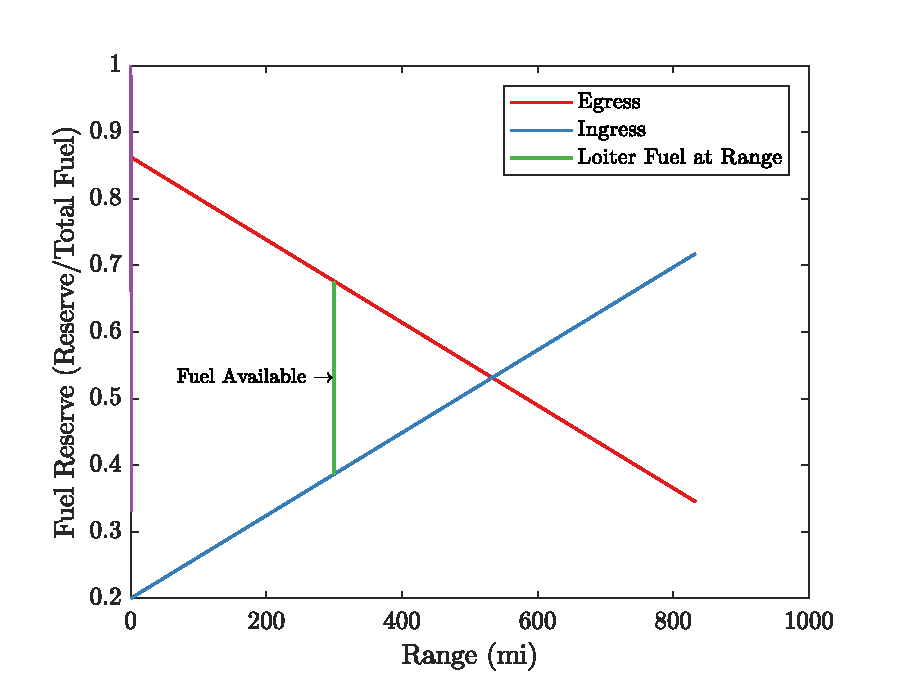
\includegraphics[width = 8cm]{Thesis/Method/ExampleFlightT37.eps}
    \caption{Example Flight Plan T-37}
    \label{fig:exT37}
\end{figure}
The non-linear equation for range is the equivalent formula presented in \ref{eq: NLRange}. The only additional parameter needed to solve for maximum range in this equation is the velocity which is assumed constant at the $C_L/C_D$. This is equivalent to finding the velocity at the maximum $\dfrac{C_L^{1/2}}{C_D}$. In the example case, since the drag polars at each mach number are unknown, a velocity of 0.5 mach at sea level will be used. Solving Eq. \ref{eq: NLRange} for fuel reserve, the egress equation becomes
\begin{equation}
    \textit{fuel remaining} = \dfrac{\exp\left[\left(\dfrac{-R}{V}\right)\dfrac{(TSFC)}{C_L/C_D}\right]W_i-\textit{dry weight}}{\textit{full weight} - \textit{dry weight}}.
\end{equation}
The equation for ingress is similarly derived as 
\begin{equation}
    \textit{fuel remaining} =\dfrac{\exp\left[\left(\dfrac{R}{V}\right)\dfrac{(TSFC)}{C_L/C_D}\right]W_i-\textit{dry weight}}{\textit{full weight} - \textit{dry weight}}.
\end{equation}
In order for the equations to accurately represent fuel reserve, the given intercept must be determined for fuel burned during climb to cruise and take-off as well as the intercept for fuel reserve required.\par

% BELOW IS EXTRACTION
Parameters for the F-15C's $C_L\text{ and }C_D$ performance are referenced in Figure \ref{fig:machSpeedByGroup}. Each line in the graph represents a mach number which is formed by the value for each coefficient of lift ($C_L$) and the associated coefficient of drag ($C_D$). These are found from historical flying data for each specific aircraft. From the matrix of these values, the lift over drag and $C_L^{1/2}/C_D$ maximums can be found. Where $C_L^{1/2}/C_D$ is maximized, the respective mach number and $C_L/C_D$ can be pulled into the model as a parameter.\par
An example of drag polar outputs from the existing model are shown in Figure (PLACE) for reference. Using 

\begin{figure}%
    \centering
    \subfloat[Lift versus drag curves for all mach numbers.]{{\includegraphics[width=7cm]{Thesis/Method/AllMachNumbers.png} }}%
    \qquad
    \subfloat[Lift versus drag curves defined by mach group.]{{\includegraphics[width=7cm]{Thesis/Method/MachSpeedByGroup.png} }}%
    \caption{Coefficients of lift versus drag for the F-15C.}%
    \label{fig:machSpeedByGroup}%
\end{figure}



    \chapter{Analysis}
    \section{Introduction}
The original model from NASIC calculates a single endurance or range of an aircraft depending on inputs from a user. This method is deemed $\pm 5\%$ accurate based on comparing the ouput to explicit mission runs from a production program. With the tradeoff frontier of the developed methodology, a series of these outputs can be estimated with given flight parameters of the aircraft. To show the differences between the estimated frontier and the original model, several data points were extracted for three different aircraft, with the last aircraft having four differing loads depending on external fuel and payload. This resulted in six tests for the developed methodology.\par
\section{Analysis Aircraft Parameters}
From an individual output from the original model, the parameters of the aircraft are derived based on the averages at certain altitudes and weights as discussed in Section \ref{section:modelUsage}. The following table describes all the parameters for each of the six aircraft used.
\begin{table}[H]
\caption{Aircraft Parameters}
\label{tab: aircraft parameters}
\resizebox{\textwidth}{!}{%
\begin{tabular}{|l|c|c|c|c|c|c|}
\hline
                             & \textbf{F-15C} & \textbf{F-16C} & \textbf{AC1-000} & \textbf{AC2-000} & \textbf{AC3-000} & \textbf{AC4-000} \\ \hline
\textbf{TSFC}                & 1.159    & 1.206    & 1.303       & 1.232      & 1.209      & 1.180      \\ \hline
\textbf{$C_L/C_D$}                 & 8.520           & 9.880           & 9.447     & 7.930            & 7.655            & 7.860             \\ \hline
\textbf{Mach}                & 0.732         & 0.791        & 0.865     & 0.830           & 0.808        & 0.759           \\ \hline
\textbf{Fuel To Cruise}      & 42738          & 26474          & 24006            & 25471            & 27780            & 33809            \\ \hline
\textbf{Distance To Cruise}  & 31.28          & 24.84          & 28.635           & 37.605           & 44.045           & 61.64            \\ \hline
\textbf{Combat Fuel}         & 688            & 402            & 402              & 402              & 402              & 402              \\ \hline
\textbf{Climb Fuel}          & 523            & 177            & 208              & 204              & 215              & 247              \\ \hline
\textbf{Percent Reserve}     & 5              & 5              & 5                & 5                & 5                & 5                \\ \hline
\textbf{Minutes Reserve}     & 20             & 20             & 20               & 20               & 20               & 20               \\ \hline
\textbf{Egress Dry Weight}   & 31262          & 20305          & 18188            & 19797            & 20062            & 19500            \\ \hline
\textbf{Egress Full Weight}  & 44710          & 27470          & 25155            & 26764            & 29211            & 35616            \\ \hline
\textbf{Ingress Dry Weight}  & 30645          & 20107          & 17879            & 17879            & 17890            & 17748            \\ \hline
\textbf{Ingress Full Weight} & 44093          & 27272          & 24846            & 24846            & 24857            & 24715            \\ \hline
\textbf{Cruise Altitude}     & 30000          & 30000          & 30000            & 30000            & 30000            & 30000            \\ \hline
\textbf{Loiter Altitude}     & 30000          & 30000          & 30000            & 30000            & 30000            & 30000            \\ \hline
\end{tabular}
}
\end{table}
The cruise and loiter altitude describe the altitude at which these parameters were derived. These are then estimated for different altitudes using US Standard Atmosphere. The ACX-000 aircraft is a dataset for which the aircraft is unknown to test whether the method is agnostic to an aircraft.

\section{Aircraft Tradeoff Comparison}
The tradeoff frontier was compared to the NASIC model using point statistics. Between three and eight points were generated from the NASIC model depending on the range and endurance ability of the aircraft. These points were generated at ten, twenty, and thirty minutes of endurance for all aircraft, but if an aircraft was able to endure longer, the points at 40, 60, 80, and 100 minutes of endurance may have also been generated. The difference statistics were computed as the average of the absolute value of the difference between the tradeoff frontier, $E$, and the NASIC model, $O$.
\begin{equation}
    D_{avg} = \dfrac{\sum_{i = 1}^n |O_i-E_i|}{n}
\end{equation}
where $n$ is the number of points generated for an aircraft. In addition, the maximum difference between an expected value from the tradeoff frontier and the NASIC model were computed for each aircraft at each altitude which is a statistic of the model's variability over different endurances.
\begin{table}[H]
\caption{Difference Statistics Between NASIC Model and Tradeoff Model}
\label{tab:diffstatistics}
\resizebox{\textwidth}{!}{%
\begin{tabular}{|l|c|c|c|c|c|c|}
\hline
                                    & \textbf{F-15C} & \textbf{F-16C} & \textbf{AC1-000} & \textbf{AC2-000} & \textbf{AC3-000} & \textbf{AC4-000} \\ \hline
\textbf{$D_{avg}$ at 30,000ft}     & 3.537          & 5.385          & 2.614            & 4.775            & 2.778            & 22.742           \\ \hline
\textbf{Max Mins at 30,000ft} & 5.790          & 9.817          & 5.151            & 4.891            & 4.154            & 23.740           \\ \hline
\textbf{$D_{avg}$ at 20,000ft}     & 3.083          & 5.403          & 2.403            & 2.628            & 5.059            & 23.496           \\ \hline
\textbf{Max Mins at 20,000ft} & 5.686          & 9.506          & 4.174            & 3.362            & 5.334            & 24.055           \\ \hline
\textbf{$D_{avg}$ at 10,000ft}     & 4.622          & 4.838          & 3.460            & 3.001            & 4.566            & 21.146           \\ \hline
\textbf{Max Mins at 10,000ft} & 5.872          & 8.772          & 5.112            & 3.568            & 4.910            & 22.710           \\ \hline
\end{tabular}%
}
\end{table}

\begin{figure}%
    \centering
    \subfloat[Comparison at 30,000 ft]{{\includegraphics[width=7cm]{Thesis/Analysis/30000f15.eps} }}%
    \qquad
    \subfloat[Comparison at 20,000 ft]{{\includegraphics[width=7cm]{Thesis/Analysis/20000f15.eps} }}%
    \qquad
    \subfloat[Comparison at 10,000 ft]{{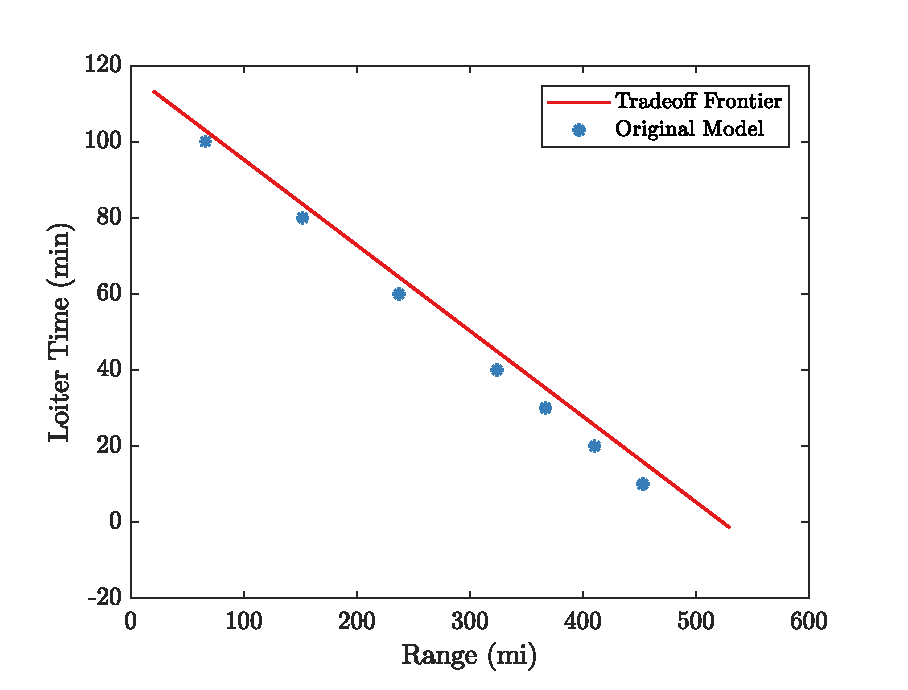
\includegraphics[width = 7cm]{Thesis/Analysis/10000f15.eps} }}
    \caption{Tradeoff Comparison for F-15C}%
    \label{fig:tradef15}
\end{figure}

\begin{figure}%
    \centering
    \subfloat[Comparison at 30,000 ft]{{\includegraphics[width=7cm]{Thesis/Analysis/30000f16.eps} }}%
    \qquad
    \subfloat[Comparison at 20,000 ft]{{\includegraphics[width=7cm]{Thesis/Analysis/20000f16.eps} }}%
    \qquad
    \subfloat[Comparison at 10,000 ft]{{\includegraphics[width = 7cm]{Thesis/Analysis/10000f16.eps} }}
    \caption{Tradeoff Comparison for F-16C}%
    \label{fig:tradef16}
\end{figure}
    \chapter{Assignment Optimization Formulation}
    \section{Introduction}
The developed methodology accounts for performance characteristics in a concise way that lends itself to optimization formulation without becoming intractable. This chapter discusses the relevance of the aircraft routing problem in literature as well as their shortcomings with respect to the inclusion of aircraft performance. Additionally, the chapter introduces several formulations in which the methodology is used to account for fuel efficiency and loiter availability at interest locations. The first two formulations explore the use of the methodology with multiple aircraft interested in traveling to multiple locations and optimizing total loiter time and priority of locations. The last formulation examines the inclusion of fuel burn on a single aircraft's path to multiple locations while loitering at each location.
\section{Aircraft Routing Optimization Literature Review}
The aircraft assignment problem is an application of the assignment problem to target locations from a starting point. A modified assignment problem can consist of one aircraft and multiple locations, a one-to-one matching of aircraft to target locations, or multiple aircraft to a greater number of locations. An assignment problem is a special case of the transportation problem where supply and demand are equal to one for all locations. The mathematical model for an assignment problem is as follows:
\begin{align}
    \min\hspace{0.5cm} &\sum_{i=1}^m\sum_{j = 1}^mc_{ij}x_{ij}\\
    \text{s.t.} \hspace{0.5cm} &\sum_{j=1}^mx_{ij} = 1, \hspace{0.5cm} \forall i \in \{1,...,m\}\\
    &\sum_{i=1}x_{ij} = 1, \hspace{0.5cm} \forall j \in \{1,...,m\}\\
    &x_{ij} \in \{0,1\}, \hspace{0.5cm} \forall i,j\in \{1,...,m\}
\end{align}
where $c_{ij}$ is the cost of assigning $i$ to $j$ and $m$ is the number of assignments \cite{bazaraa}. 
\par
A binary integer linear program (BIP) is generally the designation of assignment problems, given that the constraints and objective function are linear and that an assignment decision variable is binary-valued. In their paper on the UAV routing assignment problem, Shetty et al. \cite{Shetty} use a mixed integer linear program wherein the main constraints are service level and weaponry constraints. Their formulation serves as a traveling salesman problem (TSP), where the objective is to minimize cost, but all locations must be visited in the model. There is no upper-level constraint for ability to travel or service for any amount of time. While this formulation showcases a valid assignment problem for UAV waypoints and is similar to the way a formulation for multiple aircraft waypoints are visited, the constraints do not capture the performance characteristics of the aircraft and only seek to minimize cost rather than matching realistic performance capabilities. \par
In contrast, Alighanbari et al. \cite{Alighanbari}, Schumacher et al. \cite{Schumacher}, and Taylor et al. \cite{Taylor}, use constrained optimization based on range, timing, or fuel ratios. The advantage of this formulation is that it can represent real-world scenarios such as UAV waypoints \cite{Alighanbari} or flight mapping for commercial airliners \cite{Taylor}. Although Taylor et al. \cite{Taylor} used the TSP formulation in their model, the idea of using fuel as a constraint accounts for all possible maneuvers in an aircraft. This formulation informs the way performance characteristics of the aircraft is accounted for within constraints.\par
Vitte \cite{OptimizeBreguet} discusses the continuous coverage of a target area using a time on station designation and assuming a constant idle time. His formulation allowed for a maximization of time on station for a certain number of aircraft while meeting the constraints for turn-around time and outbound time for any particular aircraft. Integrating this idea while allowing for multiple target locations in an imperfect matching scheme allows for a decision maker to maximize the priority of targets with limited resources. While this is promising with respect to maximizing the priority of targets, the formulation lacks relevance to the performance characteristics of the aircraft used and disregards the fuel efficiency of an aircraft as it burns fuel.\par
Kannon et. al. \cite{Kannon} examines the incorporation of fuel over a series of time steps in an aircraft routing formulation. At each time step, fuel can change depending on a previous aerial refueling. Using an MILP, the formulation solves for the optimal optimal route through a series of intermediary nodes and the refueling intermediary node between a source and sink. The concept of a time step can follow the use of fuel along a route and involve how fuel efficiency changes over fuel burn. This formulation informs the way fuel is initialized as a decision variable and constrained over the course of the solution process.\par

%Missing from the lit review is how the works relate (or don't) to your own. At present, a reader doesn't know why each work is reviewed.  For a given work, is it foundational in some way?  Does it inform your model?  Does it inform your conceptual development of a model?  Or was it a promising approach that didn't quite fit your problem, so it's important to indicate how your problem differs in a way that requires a different model?
\section{Initial Formulation}
Let $x_{ij}$ be a binary variable where $x_{ij} = 1$ if plane $i$ travels to location $j$. Additionally let $d_{ij}$ be the number of miles from a starting, $i$ point to an interest location,$j$, and $E_{ij}$ be the maximum loiter time, given that aircraft $i$ has traveled to location $j$ where is calculated using Eq. \ref{eq:EnduranceWithRange} with $d_{ij}$ used as the range. A negative number in the $E_{ij}$ represents an inability for the aircraft to reach location $j$ from location $i$ and results in a penalty to the overall objective function. The sets $I$ and $J$ are represented as $I = \{1,2,\dots,n\}$ and $J = \{1,2,\dots,m\}$ where $n$ is the number of aircraft and $m$ is the number of locations. The formulation for maximizing endurance with $n$ aircraft and $m$ locations follows.\par

\begin{align}
    \max &\sum_{i\in I}\sum_{j\in J} E_{ij}x_{ij}\hspace{1cm}\\
    \text{s.t } &\sum_{i\in I} x_{ij}\leq 1\hspace{1cm} \forall j\in J\\
    &\sum_{j\in J}x_{ij} \leq 1\hspace{1cm} \forall i \in I\\
    &x_{ij}\in \{0,1\} \hspace{1cm} \forall i\in I, j\in J
\end{align}
The constraints represent a typical transportation problem where each aircraft can travel to at most one location and each location can be visited once. Using the Haversine formula and the methodology described in Section \ref{section:havMethod}, the endurance matrix is determined for an aircraft's performance parameters. \par
\section{Priority Assignment Formulation}
The priority assignment formulation is similar to the initial formulation and allows prioritizing locations. The decision for an interests point's priority is defined by the vector $\mathbf{v}$. The formulation for maximizing endurance with $n$ aircraft and $m$ locations follows.\par
\begin{equation}
    \begin{aligned}
        \max &\sum_{i\in I}\sum_{j\in J} E_{ij}v_{j}x_{ij}\hspace{1cm}\\
        \text{s.t } &\sum_{i\in I}x_{ij} \leq 1,\hspace{1cm} \forall j\in J,\\
        &\sum_{j\in J}x_{ij} \leq 1,\hspace{1cm} \forall i \in I,\\
        &x_{ij}\in \{0,1\}, \hspace{1cm} \forall i\in I, j\in J.
    \end{aligned}
\end{equation}
Though $v_j$ in this case is represented as a discrete matrix of priorities, there can also be a distribution with the endurance associated with an interest location. This broadens the ability of this formulation to utilize the developed methodology for incorporating the dynamic flight characteristics of aircraft into an assignment decision rather than a static constraint used in other literature \cite{Alighanbari,Schumacher,Taylor}.
\section{Assignment Problem Tests}
The assignment problem was tested using the aircraft parameters from AC4-000. Although the AC4-000 stressed the proposed method and incurred the most error and had the most conservative estimate from the current method, this aircraft had the longest range and, with the given list of interest points, found non-trivial solutions. The combat fuel and climb fuel were set to zero to assume that the aircraft was only interested in loiter at its respective location. The interest points were a random sequence of 100 cities in the US. All tests were run on the same 100 cities. \par
The sample problem assigned an arbitrary number of twenty aircraft to visit twenty nodes to meet the objective of maximizing total endurance. Figure \ref{fig:trivialAP} shows the results of the optimization problem run using the SCIP solver \cite{scip}.\par
\begin{figure}[H]
    \centering
    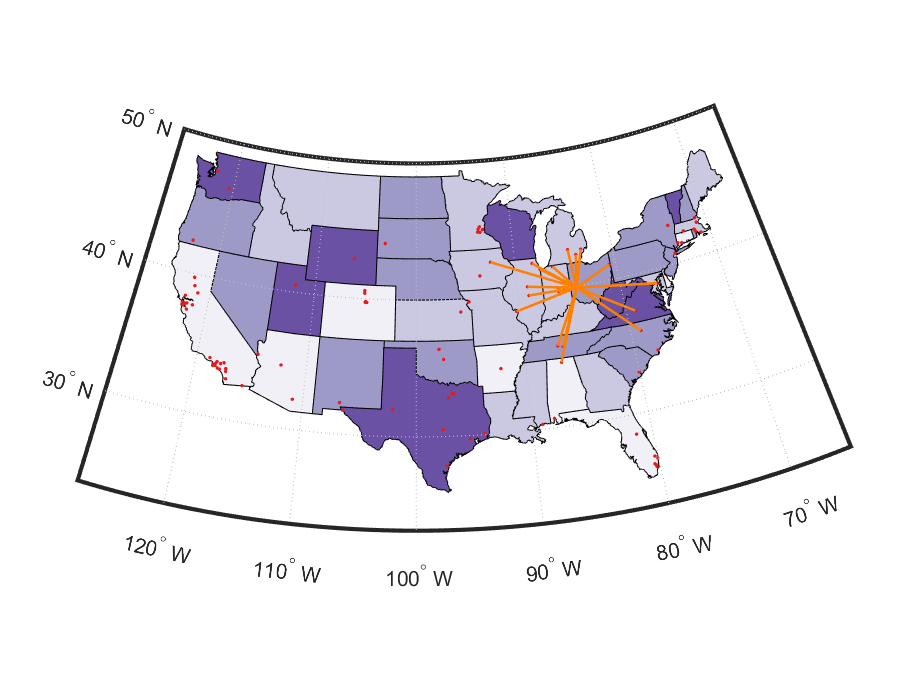
\includegraphics{Thesis/Method_II/trivialAP.eps}
    \caption{Initial Assignment Problem Example}
    \label{fig:trivialAP}
\end{figure}
As hypothesized, the results show a relatively trivial solution since all aircraft are the same and endurance at all locations is weighted equally. The twenty aircraft were assigned to the twenty nearest locations.\par
The priority assignment problem assigned a random priority to each location between zero and twenty. This test was in an attempt to determine whether a non-trivial solution can be found when certain locations are more desirable to endure over than others. The same aircraft and locations were used in this problem as in the initial assignment problem example. Figure \ref{fig:priorityAP} shows the results of the optimization problem run using the SCIP solver \cite{scip}.
\begin{figure}[H]
    \centering
    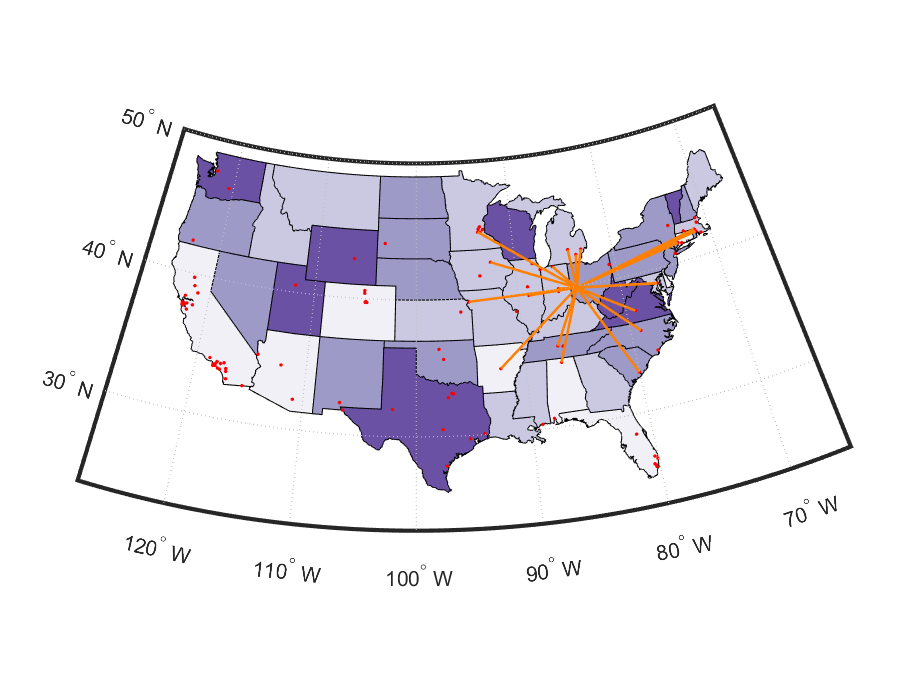
\includegraphics{Thesis/Method_II/priorityAP.eps}
    \caption{Priority Assignment Problem Example}
    \label{fig:priorityAP}
\end{figure}
The optimization problem solution verified that certain locations were a higher priority than others despite the decreased available loiter time. The aircraft traveled to locations past the previous solutions interest locations and chose to loiter at these interest points due to their higher interest.\par
Using the same optimization formulation as the priority assignment formulation, the last test was using four different aircraft, the F-15C, AC2-000, AC3-000, and AC4-000. Since these three have different endurance capabilities at their given parameters in Table \ref{tab: aircraft parameters}, the problem seeks to maximize priority while balancing the dynamic characteristics of the different aircraft. Twenty aircraft were used with five aircraft from each aircraft class. Figure \ref{fig:diffStructuresAP} shows the results of the optimization problem run using the SCIP solver \cite{scip}.
\begin{figure}[H]
    \centering
    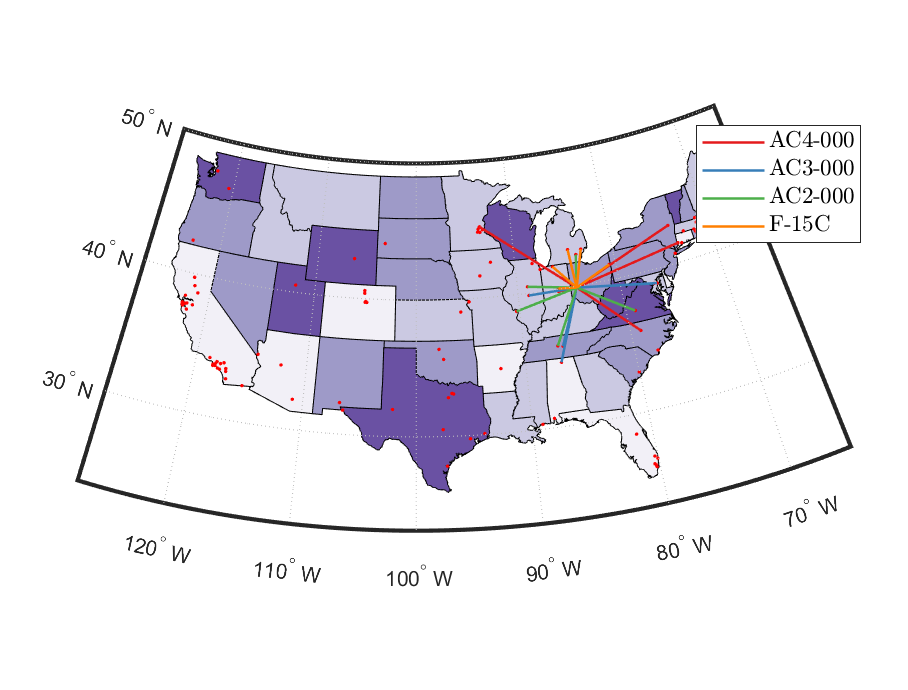
\includegraphics{Thesis/Method_II/diffStructuresAP.eps}
    \caption{Different Structures Example (with Random Priority)}
    \label{fig:diffStructuresAP}
\end{figure}
The solution showed that the aircraft with the longest range were assigned to the interest locations having both higher priorities and farther locations (AC4-000) and the shorter range aircraft were assigned to loiter over the closer distances. \par 
The assignment problem formulations successfully leveraged the methodology to quickly find a maximum loiter time over any interest location using the flight characteristics of each aircraft and in turn solve an assignment problem that maximized the interest location preferences. The solution to the priority assignment formulations were non-trivial and partitioned priority with loiter time and aircraft abilities.

\section{Decision Dependent Formulation}
\label{section:DDF}
This sub-problem seeks to route an aircraft with the given flight characteristics to multiple locations while incorporating the fuel efficiency of the nonlinear Br\'eguet range equation. The aircraft must always start from a given source node and may visit any connected node, given that the move is feasible according to its flight characteristics. The following set of parameters, decision variables, sets, and constraints define the backbone of the mixed integer nonlinear program (MINLP).
\subsection*{Parameters}
\begin{itemize}
    \item $m$ is the number of locations available to travel
    \item $D$ is a matrix of the distances between each point $D\in \mathbf{R}^{m\text{x}m}$
    \item $E$ is a matrix of efficiency factors calculated using Br\'eguet's range equation such that $E_{ij} = \exp\left[\dfrac{-D_{ij}}{V}\dfrac{TSFC}{C_L/C_D}\right]$ and $E\in \mathbf{R}^{m\text{x}m}$
    \item $s$ is both the source and sink of the model
\end{itemize}
\subsection*{Decision Variables}
\begin{itemize}
    \item $x_{ij}^{\tau}$ equals one if the aircraft travels from location $i$ to location $j$ at time decision step $\tau$
    \item $F^{\tau}$ is the amount of fuel used at decision step $\tau$
\end{itemize}
\subsection*{Sets}
\begin{itemize}
    \item $T = \{1,2,...,m\}$
    \item $I = \{1,2,...,m\}$
    \item $J = \{1,2,...,m\}$
\end{itemize}
\subsection*{Constraints}
%$\max \hspace{0.5cm} \sum \text{Endurance Utility (ie logistic curve of: $\sum(f_{ij}-R_{ij}$))}$
\begin{align}
&\sum_{j\in J} x_{sj}^{\tau} = \begin{cases} 
1, & \tau = 1,\\
0, & \forall\tau\in T-\{1\}, \end{cases} \label{cons:comefromsource}\\
&\sum_{j\in J} x_{ij}^{\tau+1}-\sum_{j\in J}x^{\tau}_{ji} = 0, \hspace{0.5cm} \forall i\in N-\{s\},\tau \in T, \label{cons:outtoin}\\
&\sum_{i\in I}x_{ii}^{\tau} = 0, \hspace{0.5cm} \forall \tau \in T, \label{cons:self}\\
&\sum_{i\in I}\sum_{\tau\in T} x_{ij}^\tau\leq 1, \hspace{0.5cm} \forall j \in J,\label{cons:do not revisit}\\
&\sum_{\tau\in T}\sum_{i\in I} x_{is}^\tau = 1,\label{cons:return}\\
&W_F-\left(\sum_{i\in I}\sum_{j\in J}E_{ij}W_Fx_{ij}^1\right) \leq F^{1}, \label{cons:fuelstart}\\
&W_F\sum_{i\in I}\sum_{j\in J}x_{ij}-\left(\sum_{i\in I}\sum_{j\in J}E_{ij}(W_F-\sum_{k = 1}^{\tau}F^{k-1})x_{ij}^{\tau}\right) \leq F^{\tau}, \hspace{.5cm} \forall \tau \in T-\{1\},\label{cons:fuelnext}\\
&\sum_{\tau\in T}\sum_{i\in I}\sum_{j\in J} F^{\tau} \leq F_{total},\label{cons:fueltotal}\\
&x_{ij}^{\tau}\in \{0,1\}, \hspace{0.5cm} \forall i\in I,j\in J,\tau\in T\label{cons:binary}.
\end{align}
Constraint \eqref{cons:comefromsource} accounts for the aircraft originating from the source node at the first decision step. Constraint \eqref{cons:outtoin} only allows the aircraft to depart from the node to which it arrived in the last decision step for all nodes except the source node since the return decision step is not known. Constraint \eqref{cons:self} does not allow the aircraft to travel to the same node at any decision step while constraint \eqref{cons:do not revisit} assures that an aircraft never departs the same node more than once in its route.  Constraint \eqref{cons:return} requires the aircraft to return to the source (once only). Constraints \eqref{cons:fuelstart} and \eqref{cons:fuelnext} incorporate the fuel burn at the start of the maneuver and for each decision step until returning to the source. Decision variable, $F^{\tau}$, is the fuel needed for the range and the additional fuel used for loiter. The variable is constrained by the aircraft's fuel burn from previous steps and needed fuel for the range given its current weight. Constraint \eqref{cons:fueltotal} ensures that the aircraft does not take a route that requires more fuel than it has in it's tank. Lastly, constraint \eqref{cons:binary} restricts the model to binary routing decisions. The nonlinearity of constraint \eqref{cons:fuelnext} differs from the typical MILP in that it requires specialized software or customized algorithms to assure that a global optimal solution is attained.\par
The objective of the decision dependent formulation is malleable in that it depends on the importance of visiting a number interest locations versus the loiter time over each interest location. Either objective can be constrained in an $\varepsilon$-constrained formulation to require a certain number of visited locations and/or a certain amount of loiter time. The former bound is the simplest constraint to implement; where the sum total of all dimensions of $x$ may be required to be greater than or equal to the number of locations. The latter bound is a harder constraint to capture in a linear form without estimating fuel burn for a certain loiter time without accounting for change in weight. A nonlinear formulation would be the most appropriate constraint for a realistic, small model, but a similar result can be obtained by constraining the minimum amount of loiter time spent at a certain location. In the next formulation, the minimum amount of fuel used for loiter time is specified by $f_{min}$.

\begin{align}
\max \hspace{0.5cm} & \sum_{\tau\in T}\sum_{i\in I}\sum_{j\in J}x_{ij}^\tau\\
\text{s.t.}\hspace{0.5cm}&\sum_{j\in J} x_{sj}^{\tau} = \begin{cases} 
1, & \tau = 1,\\
0, & \forall\tau\in T-\{1\}, \end{cases} \\
&\sum_{j\in J} x_{ij}^{\tau+1}-\sum_{j\in J}x^{\tau}_{ji} = 0, \hspace{0.5cm} \forall i\in N-\{s\},\tau \in T, \\
&\sum_{i\in I}x_{ii}^{\tau} = 0, \hspace{0.5cm} \forall \tau \in T, \\
&\sum_{i\in I}\sum_{\tau\in T} x_{ij}^\tau\leq 1, \hspace{0.5cm} \forall j \in J,\\
&\sum_{\tau\in T}\sum_{i\in I} x_{is}^\tau = 1,\\
&W_F-\left(\sum_{i\in I}\sum_{j\in J}E_{ij}W_Fx_{ij}^1\right) - F^{1}\leq -f_{min}, \\
&W_F\sum_{i\in I}\sum_{j\in J}x_{ij}-\left(\sum_{i\in I}\sum_{j\in J}E_{ij}(W_F-\sum_{k = 1}^{\tau}F^{k-1})x_{ij}^{\tau}\right) - F^{\tau}\leq \nonumber\\
&\hspace{5cm}-f_{min}*\sum_{i\in I}\sum_{j\in J}x_{ij}^\tau, \hspace{.5cm} \forall \tau \in T-\{1\},\\
&\sum_{\tau\in T}\sum_{i\in I}\sum_{j\in J} F^{\tau} \leq F_{total},\\
&x_{ij}^{\tau}\in \{0,1\}, \hspace{0.5cm} \forall i\in I,j\in J,\tau\in T.
\end{align}
Alhough the constraints are nonlinear, the solution is a realistic picture of where an aircraft should travel, given that a cruise at a lighter weight will result in a lower fuel burn than at a heavier weight. \par
The formulation of this optimization problem is tested on an arbitrary problem of five cities in the state of Ohio, Cleveland, Cincinnati, Columbus, Youngstown, and Akron. The starting node is arbitrarily chosen as Dayton, Ohio. The aircraft used in the model is the AC4-000 due to its fuel capacity. There is no combat or climb fuel used in the model to simplify the results, but the inclusion of these would be a change to the lower bound on constraint \eqref{cons:fuelstart} and constraint \eqref{cons:fuelnext}. Additionally, the aircraft does not drop its external fuel tanks or payload for model simplicity as it did in previous models.\par
The number of combinations available for values of $x$ becomes intractable as the number of locations increase. The five cities available to visit with a differing $f_{min}$ creates interesting results. Specifically, the route the aircraft takes follows paths that depend on how much fuel the aircraft burns at each location. Starting with a $f_{min}$ set at $1000$ lbs and maximizing the number of locations visited, the path follows the aircraft from Dayton to Cincinnati to Columbus to Akron to Cleveland to Youngstown and returned to Dayton. All optimization formulations were run using the SCIP solver \cite{scip}. The results are shown in Figure \ref{fig:fmin1000}.
\begin{figure}[h]
    \centering
    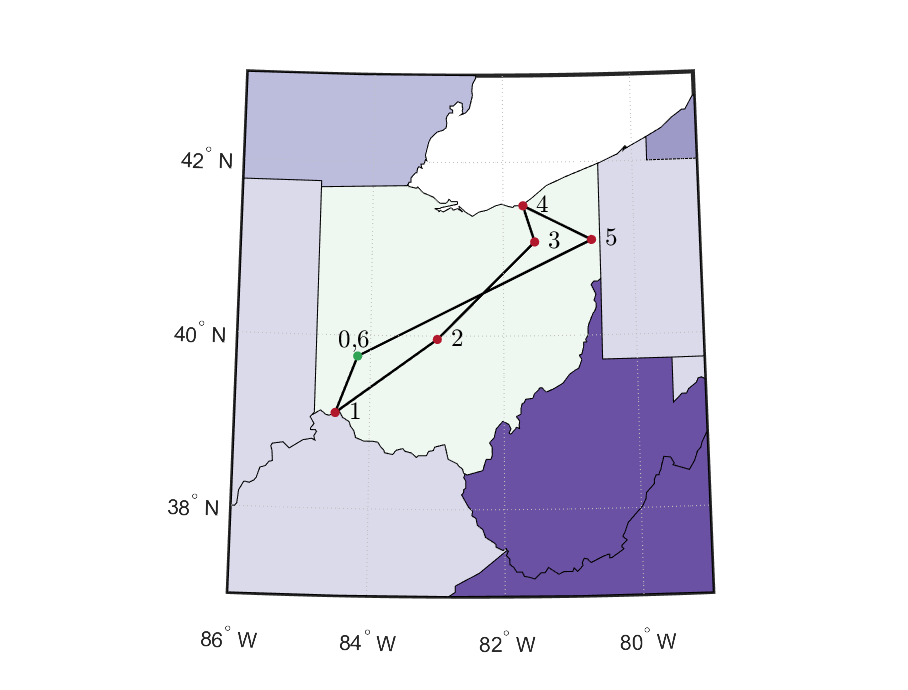
\includegraphics{Thesis/Method_II/fmin1000.eps}
    \caption{Loiter Constrained to at least 1000 lbs of Fuel}
    \label{fig:fmin1000}
\end{figure}
There are several equivalent optimal solutions as the summation of every $F^\tau$ is less than the total fuel available in the aircraft. The addition of a summation over the total fuel consumption while weighting the optimization function to also consider the number of locations visited at each time step will further incentivize the model to seek the most fuel efficient route while loitering for at least 1000 lbs of fuel which is equivalent to loitering for at least ten minutes (varying slightly due to initial weight at each location).\par
Constraining the model further to allow for at least 2200 lbs of fuel burn at each visited location gives a result where not all cities are visited. The path follows the aircraft from Dayton to Cincinnati to Columbus to Youngstown to Akron and back to Dayton. The results are shown in Figure \ref{fig:fmin2200}.
\begin{figure}[h]
    \centering
    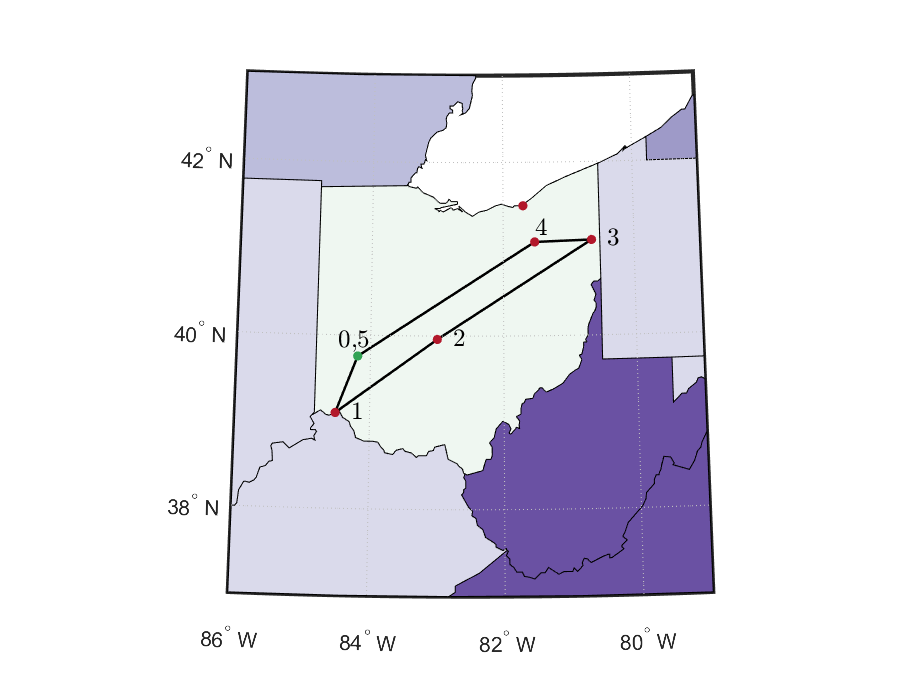
\includegraphics{Thesis/Method_II/fmin2200.eps}
    \caption{Loiter Constrained to at least 2200 lbs of Fuel}
    \label{fig:fmin2200}
\end{figure}
The formulation requires a fuel burn of 2200 lbs at each location which is equivalent to at least 25 minutes of loiter time at each location. The path follows a circular pattern that looks similar to a traveling salesman problem while excluding Cleveland. While Cleveland is closer to the starting location, Youngstown is closer to other interest locations and so the optimization chose a path to Youngstown.\par
Lastly, constraining the model by 3000 lbs of fuel burn at each location demands a loiter time of at least 35 minutes. The results are shown in Figure \ref{fig:fmin3000}.
\begin{figure}[h]
    \centering
    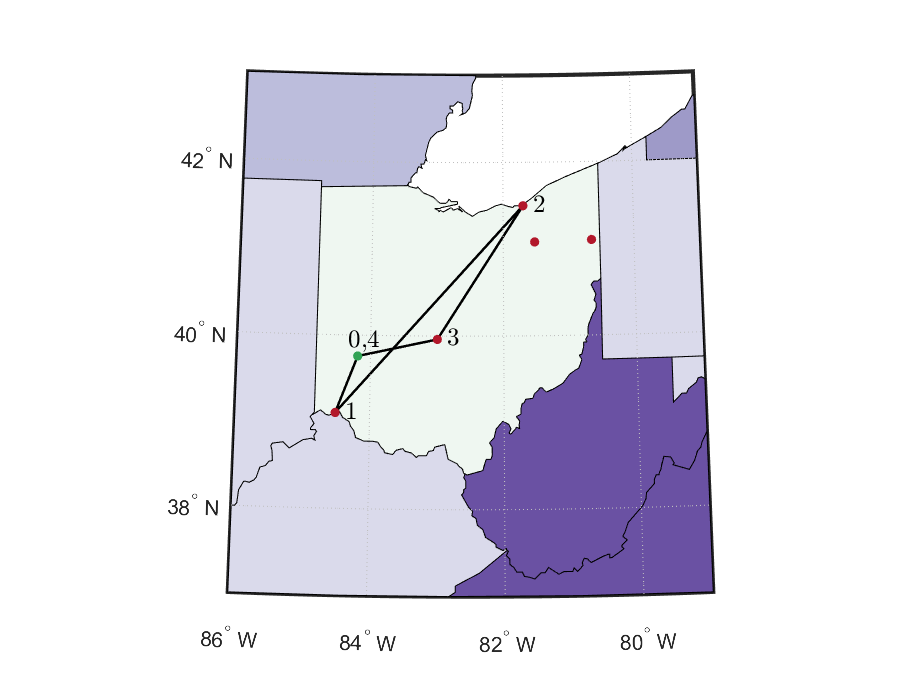
\includegraphics{Thesis/Method_II/fmin3000.eps}
    \caption{Loiter Constrained to at least 3000 lbs of Fuel}
    \label{fig:fmin3000}
\end{figure}
The path shows a more fuel efficient technique where the aircraft's path burns more fuel on its second decision and travels to Cleveland after traveling to Cincinnati in the first decision step. The path is conservative in its third and fourth decision step, traveling to Columbus and then returning to Dayton. Traveling to Akron and Youngstown is considered infeasible with the required loiter time. There are multiple optimal solutions in this scenario as there is still fuel available. Using a weighted optimization technique with an $f_{min}$ at $3000$ lbs to find the most fuel efficient route while visiting the most locations, the objective function becomes
\begin{equation}
    \max \hspace{.5cm} w_1\sum_{\tau\in T}\sum_{i\in I}\sum_{j\in J}x_{ij}^\tau-w_2\sum_{\tau\in T}F^\tau
\end{equation}
where $w_1$ and $w_2$ are arbitrary weights to scale the fuel with the binary location variable. In this example case, $w_1,w_2$ were set to 5000 and 1, respectively. The results are shown in Figure \ref{fig:weightedObj}.
\begin{figure}[h]
    \centering
    \includegraphics{Thesis/Method_II/fmin3000_negF.eps}
    \caption{Weighted Objective Function Result}
    \label{fig:weightedObj}
\end{figure}
The example shows a path from Dayton to Cleveland to Akron to Youngstown. The path chooses a cluster of the closest cities in optimizing the fuel efficiency coupled with visiting the same number of cities as in the previous scenario. Interestingly, the aircraft does not visit Columbus at the end of its path, most likely due to the efficiency of being lighter and cruising farther in the last leg.\par
The use of this technique depends on the objective function and what is desired from the MINLP model and the linear program developed in the previous subsection. The incorporation of aircraft characteristics and parameters allows for a more realistic picture of what path an aircraft could take while meeting certain requirements. 



    \chapter{Conclusion and Future Research}
    \section{Conclusion}
The proposed estimation methodology uses aircraft performance characteristics. The average difference between the tested NASIC model and the developed methodology showed that the estimation technique is effective and the tradeoff between performance metrics can be quickly estimated with one run of the model for a combination of any two of the metrics, range, loiter time, or loiter altitude, with the third held constant. This efficiency in runtime and estimation of tradeoffs is far superior to the original NASIC method which involved running individual points and linearly interpolating between results. The new method can be used to account for flight performance characteristics with a much more efficient use of resources and time.\par
The developed methodology also benefited the optimization of realistic assignment and routing problems. The nonlinear range equation was used to estimate fuel efficiency and accurately estimate a maximum range and loiter time at a given altitude and specific performance characteristics. The use of this equation in optimization is a novel approach to involving performance characteristics within the assignment and routing formulation. Incorporating the nonlinear range equation in a simple priority assignment problem allowed for a more realistic view of how an aircraft might be assigned to interest locations for loiter depending on their performance characteristics and the priority assigned to each location. Additionally, the involvement of the nonlinear range equation in accounting for fuel efficiency in an a routing formulation for a lighter aircraft indicated that a realistic approach to aircraft performance may be better served with a dynamic constraint rather than using a constant for fuel burn in optimization formulations.
\section{Future Research}
This research is heavily constrained by the estimation of aircraft performance characteristics. Since velocity, lift over drag, and thrust-specific fuel consumption are dynamic as the aircraft burns fuels, accuracy could be increased with a table lookup for each major stage of the aircraft's weight change. The nonlinear range equation estimates the dynamic performance of the aircraft, but accuracy suffers as the weight changes drastically in the cases with a payload or external fuel tank drop. Another dynamic aspect of aircraft performance is the inclusion of flight conditions. While the NASIC model also does not include these factors, the inclusion of weather, maintenance, lethal envelopes, terrain constraints and/or uncertainty would elevate the real-world relevance of the developed methodology. \par
The research's optimization section focused on small example problems for validation of the formulations. Testing the formulated optimization models against relevant literature instances would increase the validity of the model and better examine the impact of adding the dynamic fuel constraint. Efficiency of the optimization model is decreased in its nonlinear form and would also benefit from a dynamic programming approach. \par
The inclusion of several different jet aircraft allowed for additional adjustments of the model. Extending the methodology to different types of aircraft to include propeller-driven aircraft and unmanned aerial systems would be a valid extension of this model. These are referenced by different range equations and parameters. The routing assignment problem might also better serve an unmanned aerial system versus a jet aircraft due to its mission capabilities and requirements such as range and loiter time over target areas.
    \appendix
    \chapter{F-15C Parameter Extraction Data}
\renewcommand\thesection{\Alpha {A}}

\label{section:dragpolar}
\label{app: polar}
\begin{verbatim}
0F-15C                               
 GUN                                      
0POLAR DRAG OUTPUT
\end{verbatim}
\begin{figure}[H]
    \centering
    \includegraphics[width = 15cm]{Thesis/Appendices/Drag_Polar_Example.png}
    %\caption{}
    %\label{fig:my_label}
\end{figure}

\chapter{Tradeoff Comparisons}
\label{app:tradeoffComps}
\begin{figure}[H]%
    \centering
    \subfloat[Comparison at 30,000 ft]{{\includegraphics[width=5cm]{Thesis/Analysis/Tradeoff_Pics/30000f16.eps} }}%
    \qquad
    \subfloat[Comparison at 20,000 ft]{{\includegraphics[width=5cm]{Thesis/Analysis/Tradeoff_Pics/20000f16.eps} }}%
    \qquad
    \subfloat[Comparison at 10,000 ft]{{\includegraphics[width = 5cm]{Thesis/Analysis/Tradeoff_Pics/10000f16.eps} }}
    \caption{Tradeoff Comparison for F-16C}%
    \label{fig:tradef16}
\end{figure}

\begin{figure}[H]%
    \centering
    \subfloat[Comparison at 30,000 ft]{{\includegraphics[width=5cm]{Thesis/Analysis/Tradeoff_Pics/30000c1.eps} }}%
    \qquad
    \subfloat[Comparison at 20,000 ft]{{\includegraphics[width=5cm]{Thesis/Analysis/Tradeoff_Pics/20000c1.eps} }}%
    \qquad
    \subfloat[Comparison at 10,000 ft]{{\includegraphics[width = 5cm]{Thesis/Analysis/Tradeoff_Pics/10000c1.eps} }}
    \caption{Tradeoff Comparison for AC1-000}%
    \label{fig:tradec1}
\end{figure}

\begin{figure}[H]%
    \centering
    \subfloat[Comparison at 30,000 ft]{{\includegraphics[width=5cm]{Thesis/Analysis/Tradeoff_Pics/30000c2.eps} }}%
    \qquad
    \subfloat[Comparison at 20,000 ft]{{\includegraphics[width=5cm]{Thesis/Analysis/Tradeoff_Pics/20000c2.eps} }}%
    \qquad
    \subfloat[Comparison at 10,000 ft]{{\includegraphics[width = 5cm]{Thesis/Analysis/Tradeoff_Pics/10000c2.eps} }}
    \caption{Tradeoff Comparison for AC2-000}%
    \label{fig:tradec2}
\end{figure}

\begin{figure}[H]%
    \centering
    \subfloat[Comparison at 30,000 ft]{{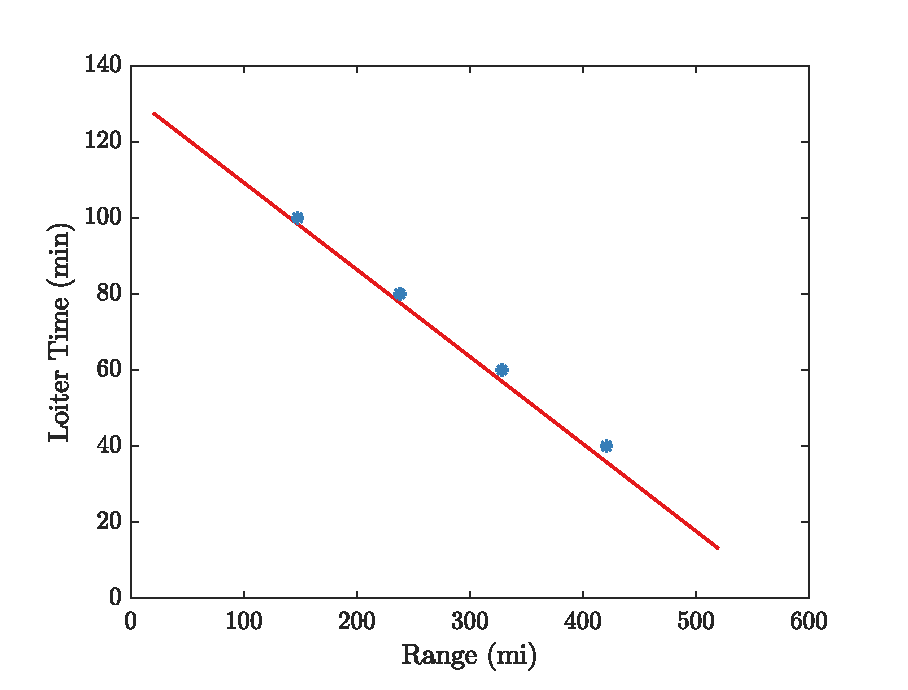
\includegraphics[width=5cm]{Thesis/Analysis/Tradeoff_Pics/30000c3.eps} }}%
    \qquad
    \subfloat[Comparison at 20,000 ft]{{\includegraphics[width=5cm]{Thesis/Analysis/Tradeoff_Pics/20000c3.eps} }}%
    \qquad
    \subfloat[Comparison at 10,000 ft]{{\includegraphics[width = 5cm]{Thesis/Analysis/Tradeoff_Pics/10000c3.eps} }}
    \caption{Tradeoff Comparison for AC3-000}%
    \label{fig:tradec3}
\end{figure}

\begin{figure}[H]%
    \centering
    \subfloat[Comparison at 30,000 ft]{{\includegraphics[width=5cm]{Thesis/Analysis/Tradeoff_Pics/30000c4.eps} }}%
    \qquad
    \subfloat[Comparison at 20,000 ft]{{\includegraphics[width=5cm]{Thesis/Analysis/Tradeoff_Pics/20000c4.eps} }}%
    \qquad
    \subfloat[Comparison at 10,000 ft]{{\includegraphics[width = 5cm]{Thesis/Analysis/Tradeoff_Pics/10000c4.eps} }}
    \caption{Tradeoff Comparison for AC4-000}%
    \label{fig:tradec4}
\end{figure}

\chapter{MATLAB Code for Structure Tradeoffs}
\renewcommand\thesection{\Alpha {A}}
\section{Linear Tradeoff Code}
\lstinputlisting[language = MATLAB]{Thesis/Appendices/Code/simpleplan.m}
\renewcommand\thesection{\Alpha {B}}
\section{Nonlinear Tradeoff Code}
\lstinputlisting[language = MATLAB]{Thesis/Appendices/Code/FixForWeight.m}
\renewcommand\thesection{\Alpha {C}}
\section{Example Structure Code}
\lstinputlisting[language = MATLAB]{Thesis/Appendices/Code/StructForNL_F15.m}

\chapter{MATLAB Code for Optimization Formulations}
\renewcommand\thesection{\Alpha {A}}
\section{Assignment Problem}
\lstinputlisting[language = MATLAB]{Thesis/Appendices/Code/AssignmentProblemTry.m}

\renewcommand\thesection{\Alpha {B}}
\section{Random Priority Assignment Problem}
\lstinputlisting[language = MATLAB]{Thesis/Appendices/Code/RandPriorityAssignment.m}

\renewcommand\thesection{\Alpha {C}}
\section{Random Priority Assignment Problem with Multiple Structures}
\lstinputlisting[language = MATLAB]{Thesis/Appendices/Code/DiffStructuresAssignmentProblem.m}

\renewcommand\thesection{\Alpha {D}}
\section{Decision Dependent Formulation}
\lstinputlisting[language = MATLAB]{Thesis/Appendices/Code/LargerDecisionDependentFormulation.m}

\renewcommand\thesection{\Alpha {E}}
\section{Decision Dependent Formulation with Constrained Loiter Fuel}
\lstinputlisting[language = MATLAB]{Thesis/Appendices/Code/ExtraConstrainedForEnduranceDDF.m}

\chapter{Python Class Method}
\renewcommand\thesection{\Alpha {A}}
\section{Aircraft Class Structure}
\lstinputlisting[language = Python]{Thesis/Appendices/Code/AircraftClass.py}

\renewcommand\thesection{\Alpha {B}}
\section{Radius and Distance Method}
\lstinputlisting[language = Python]{Thesis/Appendices/Code/RadiusCode.py}

\renewcommand\thesection{\Alpha {C}}
\section{Model Inputs Text Parser}
\lstinputlisting[language = Python]{Thesis/Appendices/Code/modelinputs.py}

\renewcommand\thesection{\Alpha {D}}
\section{Example Usage}
\lstinputlisting[language = Python]{Thesis/Appendices/Code/exampleusage.py}
\backmatter
	\singlespace
	\bibliographystyle{plain}
	\bibliography{NasicBib} 
	\clearpage
\date{March 2019}
\ReportDate{21--03--2019} \ReportType{Master's Thesis}
\DatesCovered{Jun 2018 --- Mar 2019}

\Title{\centering \MakeUppercase{AFIT/ENP Thesis Primer:}\\
                  \MakeUppercase{ a document in \LaTeX}}

%\Title{\centering \MakeUppercase{Evaluation of Interplanetary
%Magnetic Field Tracing Models Using Impulsive SEP's}}

%\ContractNumber{DACA99--99--C--9999}

%\GrantNumber{}
%\ProgramElementNumber{}
%\ProjectNumber{09ENP???}
%\TaskNumber{}
%\WorkUnitNumber{}

\Author{Lauren M. Bramblett}

\PerformingOrg{Air Force Institute of Technology\\[-1pt]
    Graduate School of Engineering and Management (AFIT/EN)\\[-1pt]
    2950 Hobson Way\\[-1pt]
    WPAFB OH 45433-7765}

\POReportNumber{AFIT--ENS--}

\SponsoringAgency{National Air and Space Intelligence Center\\[-1pt]
1940 Allbrook Drive\\[-1pt]
WPAFB OH 45433-7765\\[-1pt]}
%DSN 271-0690, COMM 937-255-3636\\[-1pt]
%Email: amy.magnus@afit.edu }

\Acronyms{NASIC}
%\SMReportNumber{}
\DistributionStatement{DISTRIBUTION STATEMENT A:\\
\MakeUppercase{Approved for Public Release; distribution unlimited.}}

\Abstract{This primer aids the AFIT student in generating the first draft of
their thesis using \Latex. The primer is produced according the tenets
described within the document.  All source code is provided in a zip
file posted to \primerAddress.  The file structure of this zip file
demonstrates a practical way to organize a thesis with its supporting
materials and---further---illustrates how your document can be produced
with version control.
}

\SubjectTerms{LaTeX,Thesis,typesetting}

\NumberPages{111}
%\ReportClassification{}
%\PageClassification{}
%\AbstractClassification{}
\AbstractLimitation{UU}

\ResponsiblePerson{Dr. L. E. Champagne, AFIT/ENS}

\RPTelephone{(937) 255-3636, x4555; lance.champagne@afit.edu}

\MakeRptDocPage

\end{document}
